\documentclass[UTF8,14pt,normal]{ctexart}
\usepackage{amsmath}
\usepackage{amsfonts,amssymb}
\usepackage{geometry}
\usepackage{graphicx}
\usepackage{float} 
\usepackage{tikz}

\geometry{a4paper,scale=0.66,top=0.8in,bottom=1.5in,left=1in,right=1in}
\title{线性代数 II(H)2022-2023 春夏期末答案}
\author{Shd0wash}
\date{\today}

\linespread{1.2}
\addtolength{\parskip}{.8em}

\begin{document}

\maketitle

\noindent{\heiti\textbf{一、}}幂零算子求 Jordan 标准型,平方根. \\

    \hangindent 2em
    \hangafter=0
    \noindent
    \textbf{1.} 参考谈之奕老师在线性代数 II(H) 2020.4.20 那一次课的讲解. 
    \[ G_{1}(0,\mathbf{A}) \enspace = \enspace \operatorname{span}\{(0,0,1)\} \qquad
    G_{2}(0,\mathbf{A}) \enspace = \enspace \operatorname{span}\{(0,1,0),(0,0,1)\} \qquad
    G_{3}(0,\mathbf{A}) \enspace = \enspace \mathbb{C}^{3}  \]
    从而:\\
    \[G_{2}(0,\mathbf{A}) \textbackslash G_{1}(0,\mathbf{A}) \enspace = \enspace \operatorname{span}\{(0,1,0)\} \qquad
    G_{3}(0,\mathbf{A}) \textbackslash G_{2}(0,\mathbf{A}) \enspace = \enspace \operatorname{span}\{(1,0,0)\} \]
    故搭成的梯子如下所示:\\
    \begin{figure}[htbp]
        \centering
        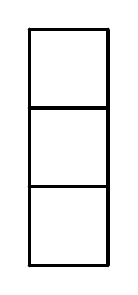
\begin{tikzpicture}
            \begin{scope}[every node/.style={thick, circle, draw, fill, scale = 0.01}]
                \node (0) at (0,0) {0};
                \node (1) at (0,1) {1};
                \node (2) at (0,2) {2};
                \node (3) at (0,3) {3};
                \node (4) at (1,0) {4};
                \node (5) at (1,1) {5};
                \node (6) at (1,2) {6};
                \node (7) at (1,3) {7};
            \end{scope}    

            \begin{scope}[every edge/.style={draw=black, very thick}]
                \path [-] (0) edge (1);
                \path [-] (1) edge (2);
                \path [-] (2) edge (3);
                \path [-] (4) edge (5);
                \path [-] (5) edge (6);
                \path [-] (6) edge (7);
                \path [-] (0) edge (4);
                \path [-] (1) edge (5);
                \path [-] (2) edge (6);
                \path [-] (3) edge (7);
            \end{scope}    
        \end{tikzpicture}
    \end{figure}

    对应的 Jordan 标准型就是 1 块 3 阶,如下:\\
    \[
    \begin{pmatrix}
        0 & 1 & 0 \\
        0 & 0 & 1 \\
        0 & 0 & 0
    \end{pmatrix}
    \]
    
    \hangindent 2em
    \hangafter=0
    \noindent
    \textbf{2.} 参考 Linear Algebra Done Right 8.A(6),采用反证法:\\
    假设存在矩阵 $ \mathbf{B} $ 使得 $ \mathbf{B}^{2} \enspace = \enspace \mathbf{A} $,则有:\\
    \[\operatorname{null} \enspace \mathbf{A}^{3} \enspace = \enspace \operatorname{null} \enspace \mathbf{B}^{6} \enspace = \enspace \operatorname{null} \enspace \mathbf{B}^{4} \enspace = \enspace \operatorname{null} \enspace \mathbf{A}^{2}\]
    由上可知这显然不等,故不存在矩阵 $ \mathbf{B} $ 使得 $ \mathbf{B}^{2} \enspace = \enspace \mathbf{A} $.

\clearpage

\noindent{\heiti\textbf{二、}}直线的位置关系.

    \hangindent 2em
    \hangafter=0
    \noindent
    形成直线 $L_{1}$ 的两个平面的法向量为 $\boldsymbol{s}_{1} \enspace = \enspace (1,1,1)$, $\boldsymbol{s}_{2} \enspace = \enspace (1,-2,0)$.\\
    $L_{1}$ 的方向向量 $l_{1} \enspace = \enspace \boldsymbol{s}_{1} \times \boldsymbol{s}_{2} \enspace = \enspace
    \begin{vmatrix}
        \boldsymbol{i} & \boldsymbol{j} & \boldsymbol{k} \\
        1 & 1 & 1 \\
        1 & -2 & 0
    \end{vmatrix} \enspace = \enspace (2,1,-3)$.\\
    $L_{2}$ 的方向向量 $l_{2} \enspace = \enspace (2,1,b)$.\\

    \hangindent 2em
    \hangafter=0
    \noindent
    \textbf{1.} $L_{1}$ 平行于 $L_{2}$,则 $\boldsymbol{l}_{1} \enspace = \enspace \lambda \boldsymbol{l}_{2}$,解得 $
    \begin{cases}
        \lambda = 1 \\
        b = -3
    \end{cases}$.\\
    取 $L_{1}$ 上一点 $A(0,1,0)$,代入 $L_{2}$ 方程发现不成立,故 $L_{1}$ 和 $L_{2}$ 不重合.\\
    所以,取 $\forall a \in \mathbb{R}, \enspace b = -3$,使得 $L_{1}$ 平行于 $L_{2}$.\\

    \hangindent 2em
    \hangafter=0
    \noindent
    \textbf{2.} 判别两直线是否异面的方法:任取 $L_{1}$ 上一点 $A$,$L_{2}$ 上一点 $B$,构成的向量 $\boldsymbol{\overrightarrow{AB}}$ 
    与 $\boldsymbol{l}_{1}$, $\boldsymbol{l}_{2}$ 作混合积,若不等于零则两直线异面,若等于零则两直线共面.\\
    取 $L_{1}$ 上一点 $A(0,1,0)$, $L_{2}$ 上一点 $B(0,a,1)$.
    $\boldsymbol{\overrightarrow{AB}}$, $\boldsymbol{l}_{1}$, $\boldsymbol{l}_{2}$ 作混合积得:\\
    \[\boldsymbol{\overrightarrow{AB}} \cdot (\boldsymbol{l}_{1} \times \boldsymbol{l}_{2}) \enspace = \enspace 
    \begin{vmatrix}
        0 & a - 1 & 1 \\
        2 & 1 & -3 \\
        2 & 1 & b
    \end{vmatrix} \enspace = \enspace -2(a - 1)(b + 3) \neq 0\]
    解得 $a \neq 1$ 且 $ b \neq -3$. \\
    所以取 $ a \neq 1, \enspace b \neq -3$时,$L_{1}$ 和 $L_{2}$ 异面.

\noindent{\heiti\textbf{三、}}内积定义验证,Gram-Schmidt 正交化,Riesz 表示定理.

    \hangindent 2em
    \hangafter=0
    \noindent
    \textbf{1.}内积需要验证的性质:\\
    \textbf{(i)} 正定性:$\forall \boldsymbol{x}, \enspace \boldsymbol{x} = (x_{1}, x_{2}, x_{3}), \enspace 
    \langle \boldsymbol{x}, \boldsymbol{x} \rangle_V = x^{2}_{1} + x^{2}_{2} + (x_{2} + x_{3})^{2} \geqslant 0$,
    当且仅当 $\begin{cases}
        x_{1} = 0 \\
        x_{2} = 0 \\
        x_{2} + x_{3} = 0
    \end{cases}$ 即 $\begin{cases}
        x_{1} = 0 \\
        x_{2} = 0 \\
        x_{3} = 0
    \end{cases}$,也就是 $\boldsymbol{x} = \boldsymbol{\theta}$ 时等号成立.\\
    \textbf{(ii)} 线性性:$\forall \boldsymbol{x}, \boldsymbol{y}, \boldsymbol{z}, \enspace 
    \boldsymbol{x} = (x_{1}, x_{2}, x_{3}), \enspace \boldsymbol{y} = (y_{1}, y_{2}, y_{3}), \enspace \boldsymbol{z} = (z_{1}, z_{2}, z_{3}), \enspace
    \forall \alpha, \beta \in \mathbb{R}$, \\
    \begin{align*}
        \langle \alpha\boldsymbol{x} + \beta \boldsymbol{z}, \boldsymbol{y} \rangle_V 
        & = (\alpha x_{1} + \beta z_{1})y_{1} + (\alpha x_{2} + \beta z_{2})y_{2} + ((\alpha x_{2} + \beta z_{2}) + (\alpha x_{3} + \beta z_{3}))(y_{2} + y_{3}) \\ 
        & = \alpha(x_{1}y_{1} + x_{2}y_{2} + (x_{2} + x_{3})(y_{2} + y_{3})) + \beta(z_{1}y_{1} + z_{2}y_{2} + (z_{2} + z_{3})(y_{2} + y_{3})) \\ 
        & = \alpha \langle \boldsymbol{x}, \boldsymbol{y} \rangle_V + \beta \langle \boldsymbol{z}, \boldsymbol{y}\rangle_V 
    \end{align*}
    \textbf{(iii)} (共轭)对称性:$\forall \boldsymbol{x}, \boldsymbol{y}, \enspace 
    \boldsymbol{x} = (x_{1}, x_{2}, x_{3}), \enspace \boldsymbol{y} = (y_{1}, y_{2}, y_{3})$
    \begin{align*}
        \langle \boldsymbol{x}, \boldsymbol{y} \rangle_V 
        & = x_{1}y_{1} + x_{2}y_{2} + (x_{2} + x_{3})(y_{2} + y_{3}) \\
        & = y_{1}x_{1} + y_{2}x_{2} + (y_{2} + y_{3})(x_{2} + x_{3}) \\ 
        & = \langle \boldsymbol{y}, \boldsymbol{x} \rangle_V 
    \end{align*}
    所以, $\langle \cdot, \cdot \rangle$ 是 $\mathbb{R}^{3}$ 上的内积.

    \hangindent 2em
    \hangafter=0
    \noindent
    \textbf{2.} 选择自然基 $\boldsymbol{e}_{1} = (1, 0, 0)$, $\boldsymbol{e}_{2} = (0, 1, 0)$, $\boldsymbol{e}_{3} = (0, 0, 1)$,进行 Gram-Schmidt 正交化. \\
    \begin{align*}
        \boldsymbol{u}_{1} = \boldsymbol{e}_{1} = (1, 0, 0), \left\lVert \boldsymbol{u}_{1} \right\rVert & = 1, \boldsymbol{\varepsilon}_{1} =\frac{\boldsymbol{u}_{1}}{ \left\lVert \boldsymbol{u}_{1} \right\rVert } = (1, 0, 0) \\ 
        \boldsymbol{u}_{2} = \boldsymbol{e}_{2} - \langle \boldsymbol{e}_{2}, \boldsymbol{\varepsilon}_{1}\rangle_V \boldsymbol{\varepsilon}_{1} = (0,1,0), \left\lVert \boldsymbol{u}_{2} \right\rVert & = \sqrt{2}, \boldsymbol{\varepsilon}_{2} =\frac{\boldsymbol{u}_{2}}{ \left\lVert \boldsymbol{u}_{2} \right\rVert } = (0, \frac{1}{\sqrt{2}}, 0) \\
        \boldsymbol{u}_{3} = \boldsymbol{e}_{3} - \langle \boldsymbol{e}_{3}, \boldsymbol{\varepsilon}_{1}\rangle_V \boldsymbol{\varepsilon}_{1} - \langle \boldsymbol{e}_{3}, \boldsymbol{\varepsilon}_{2}\rangle_V \boldsymbol{\varepsilon}_{2} = (0,-\frac{1}{2},1), \left\lVert \boldsymbol{u}_{3} \right\rVert & = \frac{1}{\sqrt{2}}, \boldsymbol{\varepsilon}_{3} =\frac{\boldsymbol{u}_{3}}{ \left\lVert \boldsymbol{u}_{3} \right\rVert } = (0, -\frac{1}{\sqrt{2}}, \sqrt{2})
    \end{align*}
    所以,$ [\boldsymbol{\varepsilon}] = (\boldsymbol{\varepsilon}_{1}, \boldsymbol{\varepsilon}_{2}, \boldsymbol{\varepsilon}_{3})$ 是 $\mathbb{R}^{3}$ 在 $\langle \cdot, \cdot \rangle$ 下的一组标准正交基.

    \hangindent 2em
    \hangafter=0
    \noindent
    \textbf{3.} 公式为 Linear Algebra Done Right 书中的 6.43.\\
    定义 $\varphi (\boldsymbol{x}) = x_{1} + 2x_{2}, \boldsymbol{x} = (x_{1}, x_{2}, x_{3})$,
    则 $\boldsymbol{\beta} = \overline{\varphi (\boldsymbol{e}_{1})}\boldsymbol{e}_{1} + \overline{\varphi (\boldsymbol{e}_{2})}\boldsymbol{e}_{2} + \overline{\varphi (\boldsymbol{e}_{3})}\boldsymbol{e}_{3} = (1, 2, -2)$\\
    即 $\boldsymbol{\beta} = (1, 2, -2)$ 时,有 $\varphi (\boldsymbol{x}) = x_{1} + 2x_{2} = \langle \boldsymbol{x}, \boldsymbol{\beta}\rangle_V$
   
\noindent{\heiti\textbf{四、}} 不变子空间的求法.

    \hangindent 2em
    \hangafter=0
    \noindent
    设该矩阵为 $ \mathbf{A} $,其特征多项式为 $p(\lambda) = (\lambda - 1)(\lambda - 2)^{2}$, 解得特征值 $\lambda_{1} = 1, \enspace \lambda_{2} = 2$ \\
    对 $\lambda_{1} = 1$, $E(\lambda_{1}, \mathbf{A}) = G(\lambda_{1}, \mathbf{A}) = \operatorname{span}\{(1, 0, 0)\}$. \\
    而对 $\lambda_{2} = 2$, $E(\lambda_{2}, \mathbf{A}) = \operatorname{span}\{(0, 1, 0)\}$, $G(\lambda_{2}, \mathbf{A}) = \operatorname{span}\{(0, 1, 0), (0, 0, 1)\}$. \\
    故,所有 $ T $-不变的子空间如下(注意转换回 $ V $ 的基):\\
    \[(1) \enspace \boldsymbol{\theta} \qquad (2) \enspace \operatorname{span}\{\boldsymbol{\varepsilon}_{1}\} \qquad  (3) \enspace \operatorname{span}\{\boldsymbol{\varepsilon}_{2}\} \qquad
    (4) \enspace \operatorname{span}\{\boldsymbol{\varepsilon}_{1}, \boldsymbol{\varepsilon}_{2}\} \qquad  (5) \enspace \operatorname{span}\{\boldsymbol{\varepsilon}_{2}, \boldsymbol{\varepsilon}_{3}\} \qquad  (6) \enspace V\]

\noindent{\heiti\textbf{五、}} 真伪判断题.

    \hangindent 2em
    \hangafter=0
    \noindent
    \textbf{1.} 伪. 由第四题即可构造反例. \\
    正确的结论是:\\
    $\forall T \in L(V)$, 若子空间 $ W \in V $ 在 $ T $ 下不变,则其补空间 $ W^{'} $ 在 $ T^{*} $ 下不变.

    \hangindent 2em
    \hangafter=0
    \noindent 
    \textbf{2.} 真. 证明如下:\\
    \begin{align*}
        \langle Tv, w \rangle & = \langle \langle v, \alpha \rangle \beta, w\rangle \\
        & = \langle v, \alpha \rangle \langle \beta, w\rangle \\
        & = \overline{\langle w, \beta \rangle} \langle v, \alpha \rangle \\
        & = \langle v, \langle w, \beta \rangle \alpha \rangle \\
        & = \langle v, T^{*}w \rangle
    \end{align*}
    即 $\forall v, \enspace \langle v, T^{*}w - \langle w, \beta \rangle \alpha \rangle = 0$,得 $T^{*}w = \langle w, \beta \rangle \alpha, \enspace \forall w$.

    \hangindent 2em
    \hangafter=0
    \noindent 
    \textbf{3.} 真. 证明如下:\\
    因为 $ T $ 是非幂零算子,所以 $ T^{n} \neq 0$, $\operatorname{null} \enspace T^{n} \neq V$,又 $ \operatorname{null} \enspace T^{n - 1} \neq \operatorname{null} \enspace T^{n - 2}$,
    结合零空间序列的性质,得 $\operatorname{null} \enspace T^{n} = \operatorname{null} \enspace T^{n-1}$,且 $dim \enspace \operatorname{null} \enspace T^{n} = dim \enspace \operatorname{null} \enspace T^{n-1} = n - 1$. \\
    又 $V = \operatorname{null} \enspace T^{n} \oplus range \enspace T^{n}$,从而 $V = \operatorname{null} \enspace T^{n - 1} \oplus range \enspace T^{n - 1}$,$\operatorname{null} \enspace T^{n - 1}$ 即为 $G(0, T)$. \\
    设 $range \enspace T^{n - 1} = U$,则 $dim \enspace U = 1$. \\
    考虑 $ T $ 在 $G(0, T)$ 上的限制 $ T|_{G(0, T)}$,其为幂零算子,且幂零指数为 $ n - 1$,故其极小多项式为 $q_{1}(\lambda) = \lambda^{n - 1}$. \\
    考虑 $ T $ 在 $ U $ 上的限制 $T|_{U}$,因为 $dim \enspace U = 1$,所以其必有实特征值(定理 9.19)且不为 0. \\
    若为 0,则 $\forall u \in U$, $(T|_{U})u = Tu = 0$,而 $\forall u \in U$, $\exists v \in V$, $T^{n - 1}v = u$,代入得 $\forall v \in V$, $T^{n}v = 0$,与 $ T $ 不是幂零算子矛盾. \\
    所以,设其特征值为 $ a $, $0 \neq a \in \mathbb{R}$,其极小多项式为 $q_{2}(\lambda) = \lambda - a$. \\
    $ T $ 的极小多项式 $q(\lambda) = q_{1}(\lambda)q_{2}(\lambda) = \lambda^{n - 1}(\lambda - a), \enspace 0 \neq a \in \mathbb{R}$ 

    \hangindent 2em
    \hangafter=0
    \noindent 
    \textbf{4.} 真. 证明如下:\\
    充分性:$\mathbf{S}_{1}\mathbf{S}_{2} = \mathbf{S}_{2}\mathbf{S}_{1}$,则 $(\mathbf{A^T} + \mathbf{A})(\mathbf{A} + \mathbf{A^T}) = (\mathbf{A} + \mathbf{A^T})(\mathbf{A^T} + \mathbf{A})$,展开后得到 $\mathbf{A}\mathbf{A^T} = \mathbf{A^T}\mathbf{A}$. \\
    又 $\mathbf{A} \in \mathbb{R}^{n \times n}$,所以 $ \mathbf{A} $ 是正规矩阵. \\
    必要性逆推即可.

    \hangindent 2em
    \hangafter=0
    \noindent 
    \textbf{5.} 伪. 本题即使条件加强为自伴依然错误. \\
    如 $ \mathbf{A} = 
    \begin{pmatrix}
        1 & 1 + i \\
        1 - i & 1
    \end{pmatrix}$,$\mathbf{A} = \overline{\mathbf{A^T}}$ 说明 $\mathbf{A}$ 是自伴的,
    但其虚部矩阵为 $\begin{pmatrix}
        0 & -1 \\
        1 & 0
    \end{pmatrix}$ 不是对称的.

\noindent{\heiti\textbf{六、}} 平方根的性质,极分解

    \hangindent 2em
    \hangafter=0
    \noindent 
    (1) $ \Rightarrow $ (2) : $ T $ 是正规算子,所以 $ TT^{*} = T^{*}T$. 而由极分解 $ T = S\sqrt{G}$,且 $ \sqrt{G} $ 是自伴算子有 $ \sqrt{G} = \sqrt{G}^{*}$.
    $ T^{*} = (S\sqrt{G})^{*} = \sqrt{G}^{*}S^{*} = \sqrt{G}S^{*}$. 故 $ SGS^{*} = S\sqrt{G}\sqrt{G}S^{*} = TT^{*} = T^{*}T = G$. 又 $S^{-1} = S^{*}$,所以 $ GS = SG $.

    \hangindent 2em
    \hangafter=0
    \noindent 
    (2) $ \Rightarrow $ (3) : $ GS = SG $, $\forall v \in E(\lambda, G), \enspace Gv = \lambda v$.
    而 $ GSv = SGv = S \lambda v = \lambda Sv$,所以 $ Sv $ 是 $ G $ 属于 $ \lambda $ 的特征向量. 从而 $ G $ 的所有特征空间 $E(\lambda, G)$ 都是 $ S $-不变的.

    \hangindent 2em
    \hangafter=0
    \noindent 
    (3) $ \Rightarrow $ (1) : $ G $ 的所有特征空间 $E(\lambda, G)$ 都是 $ S $-不变的,即 $\forall v \in E(\lambda, G), \enspace Sv \in E(\lambda, G)$. \\
    也就是 $\forall v \in E(\lambda, G), Gv = \lambda v, \enspace GSv = \lambda Sv$,从而 $GSv = \lambda Sv = S \lambda v = SGv, \enspace \forall v$. \\
    从而 $ GS = SG $,又 $S^{-1} = S^{*}$,有 $ G = SGS^{*} $. 进而 $ SGS^{*} = S\sqrt{G}\sqrt{G}S^{*} $. 而又知道 $\sqrt{G}$ 是自伴的,有 $ \sqrt{G} = \sqrt{G}^{*} $. 
    所以 $ SGS^{*} = S\sqrt{G}\sqrt{G}^{*}S^{*} = S\sqrt{G}(S\sqrt{G})^{*}$,又有极分解 $ T = S\sqrt{G} $,\\ 
    故 $T^{*}T = G = SGS^{*} = TT^{*}$,所以 $ T $ 是正规算子.
\end{document}